\documentclass[10pt]{article}
\usepackage[utf8]{inputenc}
\usepackage[T1]{fontenc}
\usepackage{amsmath}
\usepackage{amsfonts}
\usepackage{amssymb}
\usepackage[version=4]{mhchem}
\usepackage{stmaryrd}
\usepackage{graphicx}
\usepackage[export]{adjustbox}
\graphicspath{ {./images/} }

\begin{document}
\section*{Gas Turbine Design Problem - HP-1 aircraft}
\section*{A. Background}
You are to determine the thrust and fuel consumption requirements of the two engines for the hypothetical passenger aircraft, the HP-1. The twin-engine aircraft will cruise at 0.83 Mach and be capable of the following requirements:

\begin{enumerate}
  \item Takeoff at maximum gross takeoff weight $W_{\text {TO }}$ from an airport at 1.6 km pressure altitude on a hot day $\left(38^{\circ} \mathrm{C}\right)$ uses a 3650 m runway. The craft is able to maintain a $2.4 \%$ single-engine climb gradient in the event of engine failure at liftoff.
  \item It transports 253 passengers and luggage ( 90 kg each) over a still-air distance of $11,120 \mathrm{~km}$. It has 30 min of fuel in reserve at end (loiter).
  \item It attains an initial altitude of 11 km at beginning of cruise ( $\mathrm{P}_{\mathrm{s}}=1.5 \mathrm{~m} / \mathrm{s}$ ).
  \item The single-engine craft cruises at $5-\mathrm{km}$ altitude at $0.45 \mathrm{Mach}\left(\mathrm{P}_{\mathrm{s}}=1.5 \mathrm{~m} / \mathrm{s}\right)$.
\end{enumerate}

All of the data for the HP-1 contained in Example 1.2 (Mattingly book) apply. Preliminary mission analysis of the HP-1 using the methods of Ref. 12 for the 11,120-km flight with 253 passengers and luggage ( $22,770-\mathrm{kg}$ payload) gives the preliminary fuel use shown in Table 1. Analysis of takeoff indicates that each engine must produce an installed thrust of 214 kN on a hot day $\left(38^{\circ} \mathrm{C}\right)$ at 0.1 Mach and $1.6-\mathrm{km}$ pressure altitude. To provide for reasonablelength landing gear, the maximum diameter of the engine inlet is limited to 2.2 m . Based on standard design practice (see Chapter 10 of the book), the maximum mass flow rate per unit area is given by:

$$
\frac{\dot{m}}{A}=231.8 \frac{\delta_{0}}{\sqrt{\theta_{0}}} \quad(\mathrm{~kg} / \mathrm{s}) / \mathrm{m}^{2}
$$

Table 1

\begin{center}
\begin{tabular}{|l|c|c|}
\hline
Description & Distance, km & Fuel used, kg \\
\hline
Taxi &  & 200 \\
\hline
Takeoff & 330 & 840 \\
\hline
Climb and accelerate & 10,650 & 5,880 \\
\hline
Cruise & 140 & 50,240 \\
\hline
Descent $\quad 1090$ &  &  \\
\hline
\begin{tabular}{l}
Loiter \\
altitude \\
\end{tabular} 30 at 9 km & 2350 &  \\
\hline
Land and taxi &  & 600 \\
\hline
Total & 11,120 & 61,200 \\
\hline
\end{tabular}
\end{center}

Thus on a hot day $\left(38^{\circ} \mathrm{C}\right)$ at 0.1 Mach and 1.6 km pressure altitude, $\theta=(38+273.1) / 288.2=$ $1.079, \theta_{0}=1.079 \times 1.002=1.081, \delta=0.8256, \delta_{0}=0.8256 \times 1.007=0.8314$, and the maximum mass flow through the 2.2 m diameter inlet is $704.6 \mathrm{~kg} / \mathrm{s}$.

\section*{B. Preliminary Calculations}
\begin{enumerate}
  \item If the HP-1 starts out the cruise at 11 km with a weight of $1,577,940 \mathrm{~N}$, find the allowable TSFC for the distance of $10,650 \mathrm{~km}$ for the following cases:\\
(a) Assume the aircraft performs a cruise climb (flies at a constant $C_{D} / C_{L}$ ). What is its altitude at the end of the cruise climb?\\
(b) Assume the aircraft cruises at a constant altitude of 11 km . Determine $C_{D} / C_{L}$ at the start and end of cruise. Using the average of these two values, calculate the allowable TSFC.
  \item Determine the loiter (endurance) Mach numbers for altitudes of 10, 9, 8, 7, and 6 km when the HP-1 aircraft is at $64 \%$ of $\mathrm{W}_{\text {TO }}$.
  \item Determine the aircraft drag at the following points in the HP-1 aircraft's $11,120 \mathrm{~km}$ flight based on the fuel consumptions just listed:\\
(a) Takeoff, $M=0.23$, sea level\\
(b) Start of cruise, $\mathrm{M}=0.83,11 \mathrm{~km}$\\
(c) End of cruise climb, $\mathrm{M}=0.83$, altitude $=$ ? km\\
(d) End of 11-km cruise, $\mathrm{M}=0.83,11 \mathrm{~km}$\\
(e) Engine out ( $88 \%$ of $\mathrm{W}_{\text {TO }}$ ), $\mathrm{M}=0.45,5 \mathrm{~km}$
\end{enumerate}

\section*{C. Parametric cycle analysis of ideal engine}
You are to determine the range of compressor pressure ratios and bypass ratios for ideal turbofan engines that best meet the design requirements for the hypothetical passenger aircraft, the HP-1.

\section*{C1. Hand-Calculate Ideal Performance (HP-1 Aircraft).}
Using the parametric cycle analysis equations for an ideal turbofan engine with $\mathrm{T}_{\mathrm{t} 4}=\ldots \mathrm{K}$, hand-calculate the specific thrust and thrust specific fuel consumption for an ideal turbofan engine with a compressor pressure ratio of $\pi_{c}=\ldots$, fan pressure ratio of $\pi_{f}=\ldots$, and bypass ratio of $\Phi=\ldots$ at the 0.83 Mach, 11 km -altitude cruise condition. Assume $\gamma=1.4, C_{p}=1.004$ $\mathrm{kJ} /(\mathrm{kg} . \mathrm{K})$, and $\mathrm{h}_{\mathrm{PR}}=42,800 \mathrm{~kJ} / \mathrm{kg}$. Compare your answers to results from the parametric cycle analysis computer programs.

\section*{C2. Computer-Calculated Ideal Performance (HP-1 Aircraft).}
For the 0.83 Mach, 11 km -altitude cruise condition, determine the performance available from turbofan engines. This part of the analysis is accomplished by using the computer program with the assigned value of $\mathrm{T}_{\mathrm{t} 4}=\ldots \mathrm{K}$. Specifically, you are to vary the compressor pressure ratio from 20 to 40 in increments of 2 . Fix the fan pressure ratio at your assigned value of $\pi_{f}=\ldots$. Evaluate bypass ratios of $4,6,8,10,12$, and the optimum value. Assume $\gamma$ $=1.4, c_{p}=1.004 \mathrm{~kJ} /(\mathrm{kg} . \mathrm{K})$, and $\mathrm{h}_{\mathrm{PR}}=42,800 \mathrm{~kJ} / \mathrm{kg}$.

C3. Calculate Minimum Specific Thrust at Cruise (HP-1 Aircraft).

You can calculate the minimum uninstalled specific thrust at cruise based on the following information:

\begin{enumerate}
  \item The thrust of the two engines must be able to offset drag at 0.83 Mach and 11 km altitude and have enough excess thrust for $P_{s}$ of $1.5 \mathrm{~m} / \mathrm{s}$. Determine the required installed thrust to attain the cruise condition using Eq. (1.28) from the book. Assuming $\Phi_{\text {inlet }}+\Phi_{\text {noz }}=0.02$, determine the required uninstalled thrust.
  \item Determine the maximum mass flow into the 2.2 m diameter inlet for the 0.83 Mach, 11 km altitude flight condition, using the equation given in the background section for this design problem in Chapter 1.
  \item Using the results of steps 1 and 2, calculate the minimum uninstalled specific thrust at cruise.
  \item Perform steps 2 and 3 for inlet diameters of 2.5, 2.75, 3.0, 3.25, and 3.5 m .
\end{enumerate}

\section*{C4. Select Promising Engine Cycles (HP-1 Aircraft).}
Plot thrust specific fuel consumption vs specific thrust (thrust per unit mass flow) for the engines analyzed in the preceding. Plot a curve for each bypass ratio, and cross-plot the values of the compressor pressure ratio (see Fig. 1). The result is a carpet plot (a multivariable plot) for the cruise condition. Now draw a dashed horizontal line on the carpet plot corresponding to the maximum allowable uninstalled thrust specific fuel consumption $\mathrm{S}_{\text {max }}$ for the cruise condition (determined in the part B of this design problem). Draw a dashed vertical line for each minimum uninstalled specific thrust determined in the preceding. Your carpet plots will look similar to the example shown in Fig. 1. What ranges of bypass ratio and compressor pressure ratio look most promising?\\
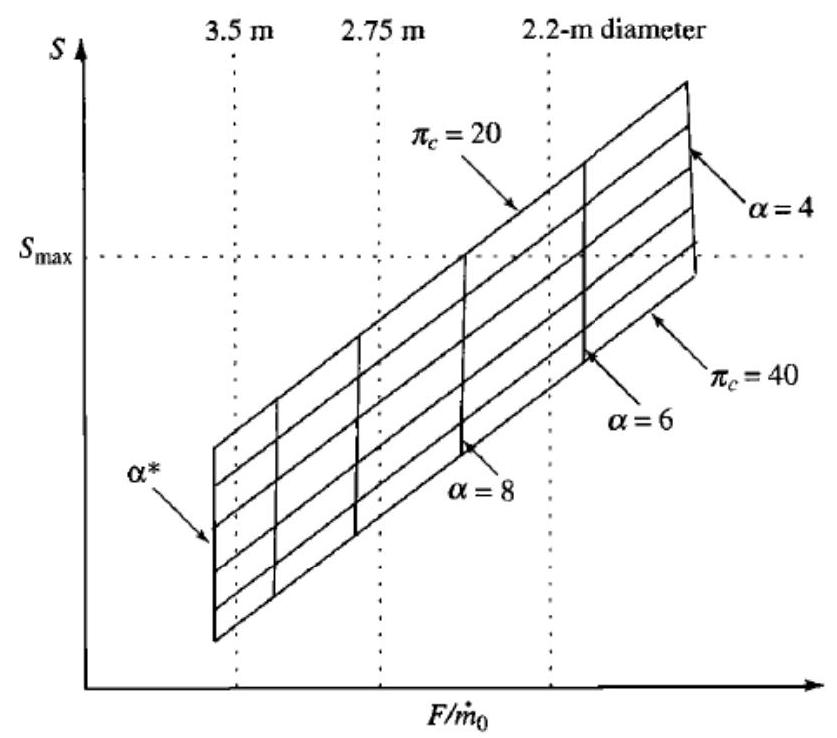
\includegraphics[max width=\textwidth, center]{plot-S-Fm}

Figure 1 Example carpet plot for HP-1 aircraft engine

\section*{D. Parametric Cycle Analysis of Real Engines}
You are to determine the range of compressor pressure ratios and bypass ratios for turbofan engines with losses that best meet the design requirements for the hypothetical passenger aircraft HP-1.

D1. Hand-Calculate Performance with Losses (HP-1 Aircraft).\\
Using the parametric cycle analysis equations for a turbofan engine with losses and component technology level 4 in Table 6.2 (assume cooled turbine, type A diffuser, and type D nozzle) with the assigned value of $\mathrm{T}_{\mathrm{t} 4}=\ldots \mathrm{K}$, hand calculate the specific thrust and thrust specific fuel consumption for a turbofan engine with a compressor pressure ratio of $\pi_{c}=\ldots$, fan pressure ratio of $\pi_{f}=\ldots$, and bypass ratio of $\alpha=\ldots$, at the 0.83 Mach and 11 km altitude cruise condition. Assume $\gamma_{\mathrm{c}}=1.4, \mathrm{C}_{\mathrm{pc}}=1.004 \mathrm{~kJ} /(\mathrm{kg} . \mathrm{K}), \gamma_{\mathrm{t}}=1.3, \mathrm{C}_{\mathrm{pt}}=1.235 \mathrm{~kJ} /(\mathrm{kg} . \mathrm{K})$, $\mathrm{h}_{\mathrm{PR}}=$ $42,800 \mathrm{~kJ} / \mathrm{kg}$, and $\eta_{\mathrm{m}}=0.99$. Compare your answers to results from the parametric cycle analysis programs PARA and part C.

\section*{D2. Computer-Calculated Performance with Losses (HP-1 Aircraft).}
For the 0.83 Mach and 11 km altitude cruise condition, determine the performance available from turbofan engines with losses. This part of the analysis is accomplished by using the computer programs with component technology level 4 in Table 6.2 (assume cooled turbine, type A diffuser, and type D nozzle) and $\mathrm{T}_{\mathrm{t} 4}=\ldots$ K. Specifically, you are to vary the compressor pressure ratio from 20 to 40 in increments of 2 . Fix the fan pressure ratio at your assigned value of $\pi_{f}=\ldots$. Evaluate bypass ratios of $4,6,8,10,12$, and the optimum value. Assume $\gamma_{\mathrm{c}}=1.4, \mathrm{c}_{\mathrm{pc}}=1.004 \mathrm{~kg} /(\mathrm{kg} . \mathrm{K}), \gamma_{\mathrm{t}}=1.3, \mathrm{c}_{\mathrm{pt}}=1.235 \mathrm{~kJ} /(\mathrm{kg} \cdot \mathrm{K}), \mathrm{h}_{\mathrm{PR}}=42,800 \mathrm{~kJ} / \mathrm{kg}$, and $\eta_{m}=0.99$.

\section*{D3. Calculate Minimum Specific Thrust at Cruise (HP-1 Aircraft).}
You can calculate the minimum uninstalled specific thrust at cruise based on the following information:

\begin{enumerate}
  \item The thrust of the two engines must be able to offset drag at 0.83 Mach and 11 km altitude and have enough excess thrust for $P_{s}$ of $1.5 \mathrm{~m} / \mathrm{s}$. Determine the required installed thrust to attain the cruise condition, using Eq. (1.28). Assuming $\Phi_{\text {inlet }}+\Phi_{\text {noz }}=0.02$, determine the required uninstalled thrust.
  \item Determine the maximum mass flow into the 2.2 m diameter inlet for the 0.83 Mach and 11 km altitude flight condition, using the equation given in the background section for this design problem in Chapter 1.
  \item Using the results of steps 1 and 2, calculate the minimum uninstalled specific thrust at cruise.
  \item Perform steps 2 and 3 for inlet diameters of 2.5, 2.75, 3.0, 3.25, and 3.5 m .
\end{enumerate}

\section*{D4. Select Promising Engine Cycles (HP-1 Aircraft)}
Plot thrust specific fuel consumption vs specific thrust (thrust per unit mass flow) for the engines analyzed in the preceding. Plot a curve for each bypass ratio and cross-plot the\\
values of the compressor pressure ratio (see Fig. 1). The result is a carpet plot (a multivariable plot) for the cruise condition. Now draw a dashed horizontal line on the carpet plot corresponding to the maximum allowable uninstalled thrust specific consumption ( $\mathrm{S}_{\mathrm{max}}$ ) for the cruise condition (determined in the A portion of this design problem). Draw a dashed vertical line for each minimum uninstalled specific thrust determined in the preceding. Your carpet plots will look similar to the example shown in Fig. 1. What ranges of bypass ratio and compressor pressure ratio look most promising? Compare to the results of part C.


\end{document}